
%%%%%%%%%%%%%%%%%%%%%%%%%%%%%%%%%%%%%%%%%%%%%%
\section{Photon detection system}

The scope of the photon detector (PD) system for the DUNE far detector
reference design includes design, procurement, fabrication,
testing, delivery and installation of the following components:
\begin{itemize}
\item light collection system including wavelength shifter and light guides,
\item silicon photo-multipliers (SiPMs),
\item readout electronics,
\item calibration system, and
\item related infrastructure (frames, mounting boards, etc.).
\end{itemize}

LAr is an excellent scintillating medium and the photon detection
system will exploit this property in the far detector.  With an
average energy of 19.5~eV needed to produce a photon (at zero field),
a typical particle depositing 1~MeV in LAr will generate
40,000~photons with wavelength of 128~nm. At higher fields this will
be reduced, but at 500~V/cm the yield is still $\sim$20,000~photons
per MeV. Roughly 1/4 of the photons are promptly emitted with a
lifetime of about 6~ns while the rest have a lifetime of
1100--1600~ns. Prompt and delayed photons are detected in
  precisely the same way by the photon detection system. LAr is
highly transparent to the 128-nm VUV photons with a Rayleigh
scattering length of (66~$\pm$~3)~cm~\cite{Rayleigh} and absorption
length of $>$200~cm; this attenuation length requires a LN2
  content of less than 20~ppm. The relatively large light yield makes
the scintillation process an excellent candidate for determination of
$t_0$ for non-beam related events. Detection of the scintillation
light may also be helpful in background rejection and triggering on
non-beam events.

The photon detection system reference design described in this section
meets the required performance for light collection for the DUNE far
detector. This includes detection of light from proton decay
candidates (as well as beam neutrino events) with high efficiency to
enable 3D spatial localization of candidate events. The TPC will
provide supernova neutrino detection. 
The photon system will provide the $t_0$ timing of
events relative to TPC timing with a resolution better than 1~$\mu$s
(providing position resolution along drift direction of a couple of mm). 

Figure~\ref{fig:PD_overview} shows the layout for the photon detector
system, which will be described in the following sections.
\begin{cdrfigure}[Photon detection system overview]{PD_overview}{Overview of the PD
    system showing a cartoon schematic (a) of a single PD module
    in the LAr and the channel ganging scheme used to reduce the
    number of readout channels. Panel (b) shows how each PD module
    will be inserted into an APA frame. There will be 10 PDs instered
    into an APA frame.}
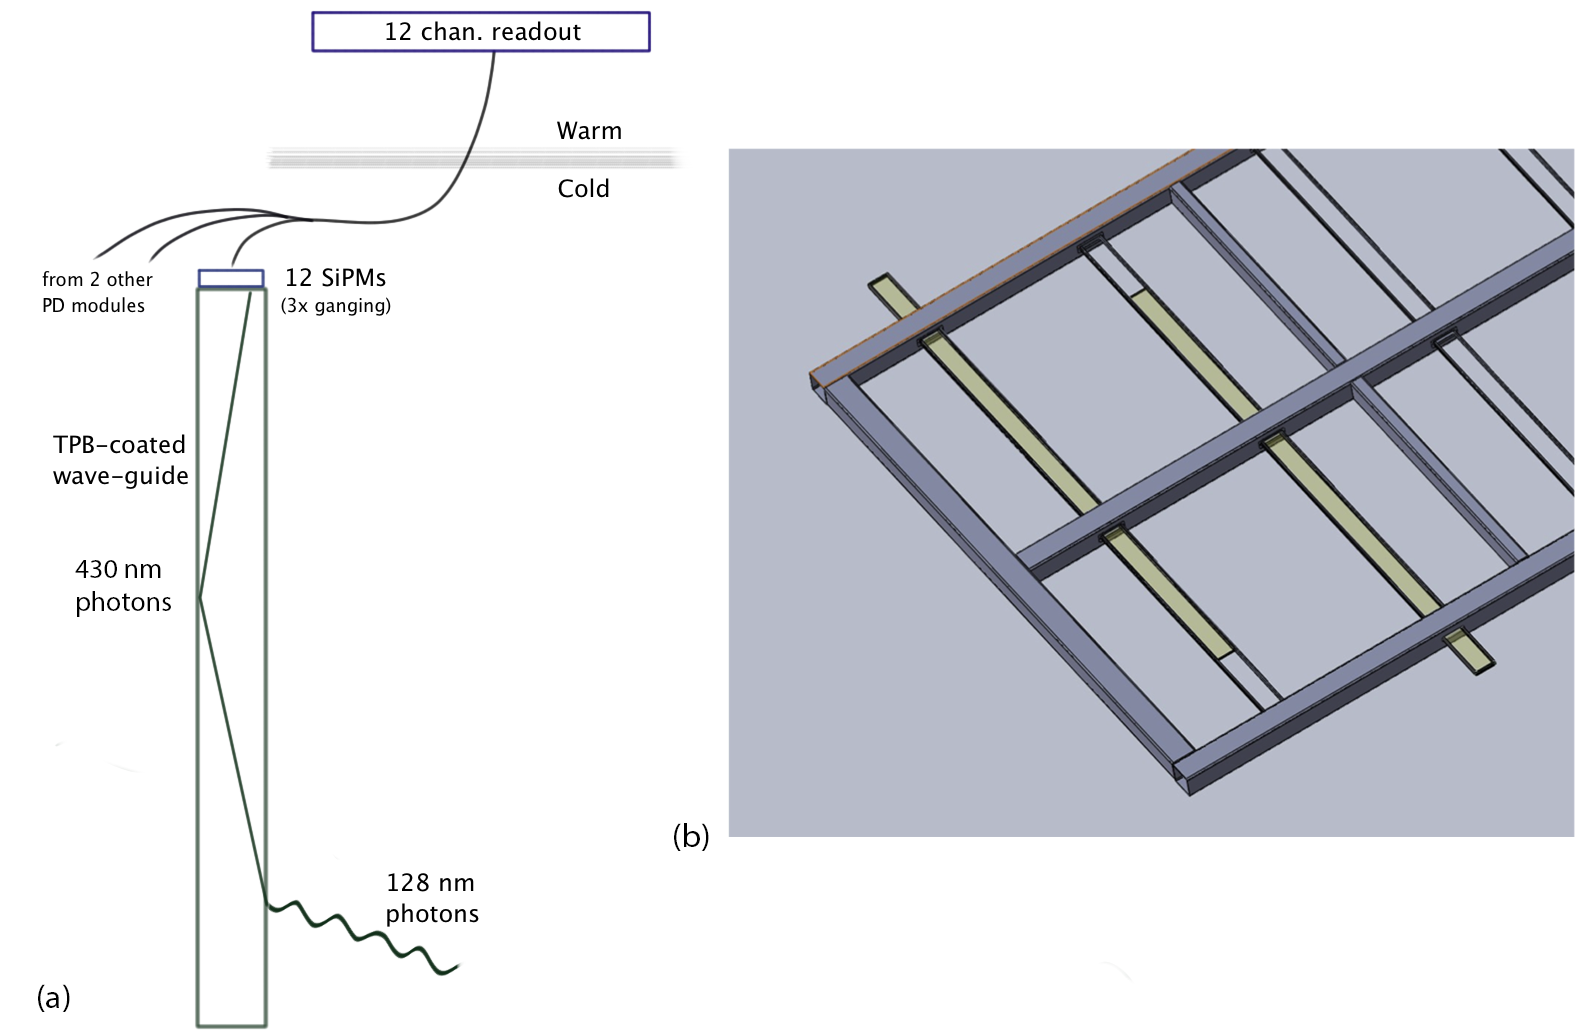
\includegraphics[width=1.0\linewidth]{pd_schem.png}
\end{cdrfigure}

%%%%%%%%%%%%%%%%%%%%%%%%%%
\subsection{Photon Detector Modules}

There are two styles of photon detector (PD) modules being produced for protoDUNE.  
The concepts are very similar, but differ in the number of times the LAr scintillation 
light is shifted.  

The reference design shown schematically in figure~\ref{fig:PD_RadiatorBar}
has wavelength shifting radiator plates mounted on a wavelength shifting light guide.
The plates are coated 
with tetraphenyl-butadiene (TPB) to produce blue ($430nm$) light from the $128nm$ VUV 
scintillation light.  
This blue light is absorbed by a commercially produced wavelength shifting (WLS)
polystyrene bar with Y-11 fluor.  
The bar serves as a light guide to transmit the green light to the photodetector 
mounted at the end.
The radiator plates are captive in mounting blocks that are glued to the WLS bar
at regular intervals as shown in figure~\ref{fig:PD_radiator_mount}.
\begin{cdrfigure}[Radiator Plate Mounting Blocks]{PD_radiator_mount}
  {Mounting of the radiator plates to the WLS bar for the reference design scheme}
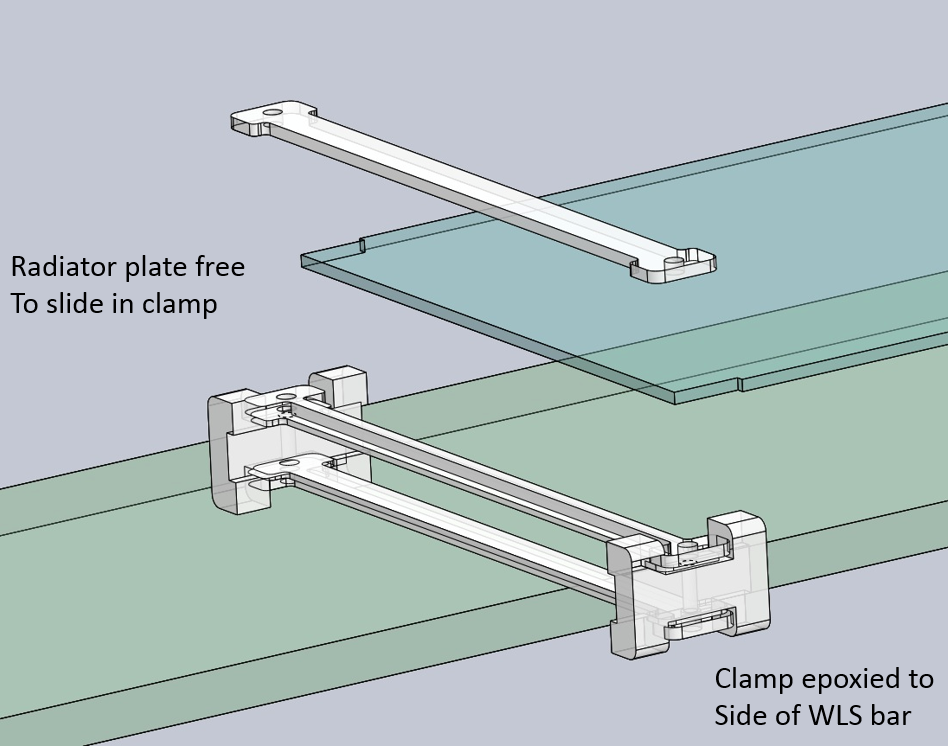
\includegraphics[width=1.0\linewidth]{PD_radiator_mount.PNG}
\end{cdrfigure}

The alternative design uses the same photodetector and mounting, but does not have
any radiator plates mounted on it.  
Instead, the bar is made by dip-coating an acrylic light guide with a solution
of TPB, solvents, and a surfactant to produce a bar with the wavelength shifter coated
on the outside.  
This has advantages in that the expensive fluor is only on the outside where it is
needed, instead of a dopant added during the casting process.  
It also only has one wavelength shifting step, and should be more efficient because
of this.  
Previous work for DUNE with this technique showed that the attenuation length, and
therefore light yield would suffer from the coating process, but bars produced with
the latest technique as shown in~\cite{conrad_jinst} have been shown to have avoided
this problem.

%%%%%%%%%%%%%
\subsubsection{Rel Light yield of alternatives}
      -IU Tallbo -- Denver/Stuart
     Results of testing
     Fit to Determine Light Yield
     Fit/Ratio vs. Distance to determine atten length     

%%%%%%%%%%%%%
\subsubsection{Absolute light yield}
     Connection to Absolute -- Tallbo-35T  -- Denver Tallbo, Celio,Jonathan,Alex --35T
     (This could get dropped, or altered depending on status of 35T)
     Light yield by paddle
     Comparison to Simulation
     pe's / MeV 

%%%%%%%%%%%%%%%%%%%%%%%%%%
\subsection{Radiator/guide lifetime}
     IU Tallbo and SDSM and T  -- IU design SDSM and T testing  CSU QA/QC
     Design/Mfr Radiator and guide
     Design/Mfr dipped guide -- Toups
     Testing - cryogenic cycling 
          rad
          guide
          dipped guide
     QA/QC tracking and testing plan  

%%%%%%%%%%%%%%%%%%%%%%%%%%
\subsection{Sensors}
The planned photodetector is a SiPM.  
The model planned for protoDUNE is the SensL C-Series 6~mm$^2$
(MicroFB-60035-SMT) devices. These SiPMs have detection efficiency of
41\%; the detection efficiency combines QE and effective area
  coverage accounting for dead space between pixels. While the
C-Series SensL SiPMs are not rated for operation below
$-$40$^{\circ}$~C their performance has been excellent for this
application. 
They have been used in several tests at Fermilab test facilities,
TallBo and Blanche, and were used for the 35T prototype detector
as well.  At LAr temperature (89~K) the dark rate is of order 10~Hz
(0.5 p.e. threshold) while after-pulsing has not been an
issue. Extensive testing is underway and will continue, to ensure 
that the SiPMs can reliably survive the stresses associated with 
any thermal cycling in LAr and long-term operation at LAr temperature.

%%%%%%%%%%%%%
\subsubsection{SiPM performance and testing}

All photodetectors for protoDUNE will be subjected to testing to determine:
\begin{itemize}
\item Photodetector Gain Curve
\item Noise rate
\item Crosstalk estimation
\item Breakdown Voltage
\end{itemize}
All items will be tested both warm and cold (cyrogenic temperature) to 
determine the operating characteristics when they will be installed at
the protoDUNE detector, and during QA/QC tests on the PD modules.

In addition to these tests, the photodetectors will be tested for their
response to light signals from an LED with appropriate wavelength.
These tests will be sensitive enough to determine if one of the 3 SiPM
elements in parallel is not functioning.

%%%%%%%%%%%%%
\subsubsection{SiPM Lifetime}
Aging studies have been performed to investigate the aging of the devices at 
cryogenic temperatures as a result of exposure to light over time.
Currently, a set of 63 devices have been tested for degradation.
The SensL Series C SiPMs showed no evidence for degradation in their 
performance in the equivalent of 250 years of exposure underground at DUNE. 
The tests investigated SiPM response, noise rate, cross-talk probability, and
gain.
Detailed test results can be seen on DUNE-doc-904. (Make a reference) 
Additional long-term testing with an expanded throughput are beginning
now.

A passive aging test was initiated in March 2015 to follow the
behavior of six SensL series C SiPMs in a simulation of the benign
DUNE environment. These SiPMs have been continuously in the
dark in LN2 for over 425 days. Four properties have been monitored:
dark noise rate, cross talk probability, breakdown voltage, and gain
slope. So far, the measurements show that there
have been no significant changes in these properties during the
duration of the test.
Detailed test results can be found in DUNE-doc-905. (make a reference)

%%%%%%%%%%%%%%%%%%%%%%%%%%
\subsection{Mechanical design and installation}
     % -- CSU  -- Dave

   %  Mechanical Design Mounting 

The PD system is mounted as modules on the APA frames.  A PD module is
the combination of one light-guide (also called a ``bar'' due to its
shape) and 12 SiPMs, as shown in Figure~\ref{fig:PD_overview}~(a).  To
enable this, the the reference design for mounting the PDs onto the
APA frames calls for ten PD modules per APA, approximately 2.2-m long,
86-mm wide and 6-mm thick, equally spaced along the full length of the
APA frame, as shown in Figure~\ref{fig:PD_overview}~(b). 
The light guides are inserted into the APA frame on rails gliding on their radiator
plate mounting blocks as shown in figure~\ref{fig:PD_mounting_inslide.PNG}.
\begin{cdrfigure}[Diagram of PD installation into APA frame]
  {PD_mounting_inslide}{Rendering of the installation of a PD module
    into an APA frame, shown just before it comes to rest on the inside face
    of the APA tube.}
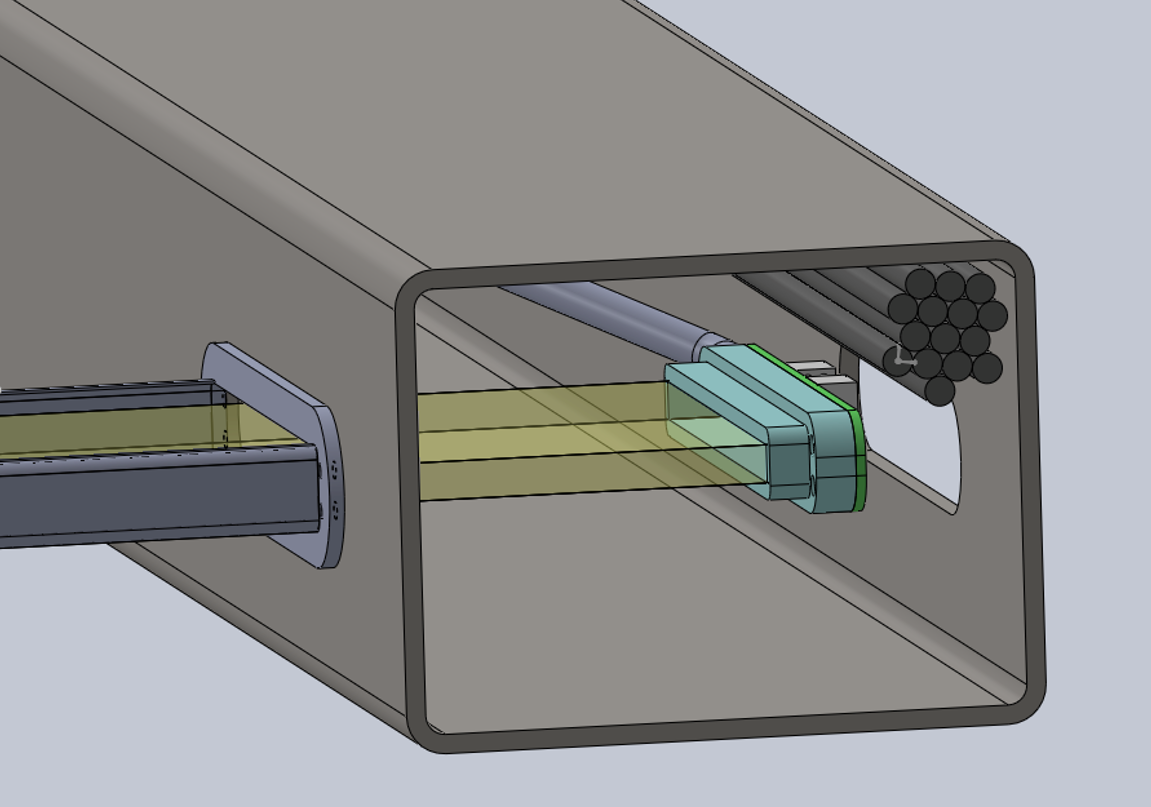
\includegraphics[width=0.50\linewidth]{PD_mounting_inslide.PNG}
\end{cdrfigure}

The system has been prototyped and test fitted with a module at CSU 
as shown in Figure~\ref{fig:PD_flat_installtest}.
\begin{cdrfigure}[Photo of PD mock installation]
  {PD_flat_installtest}{Photograph of the installation
    test of a mock PD module in a 1/5 section of an APA frame.}
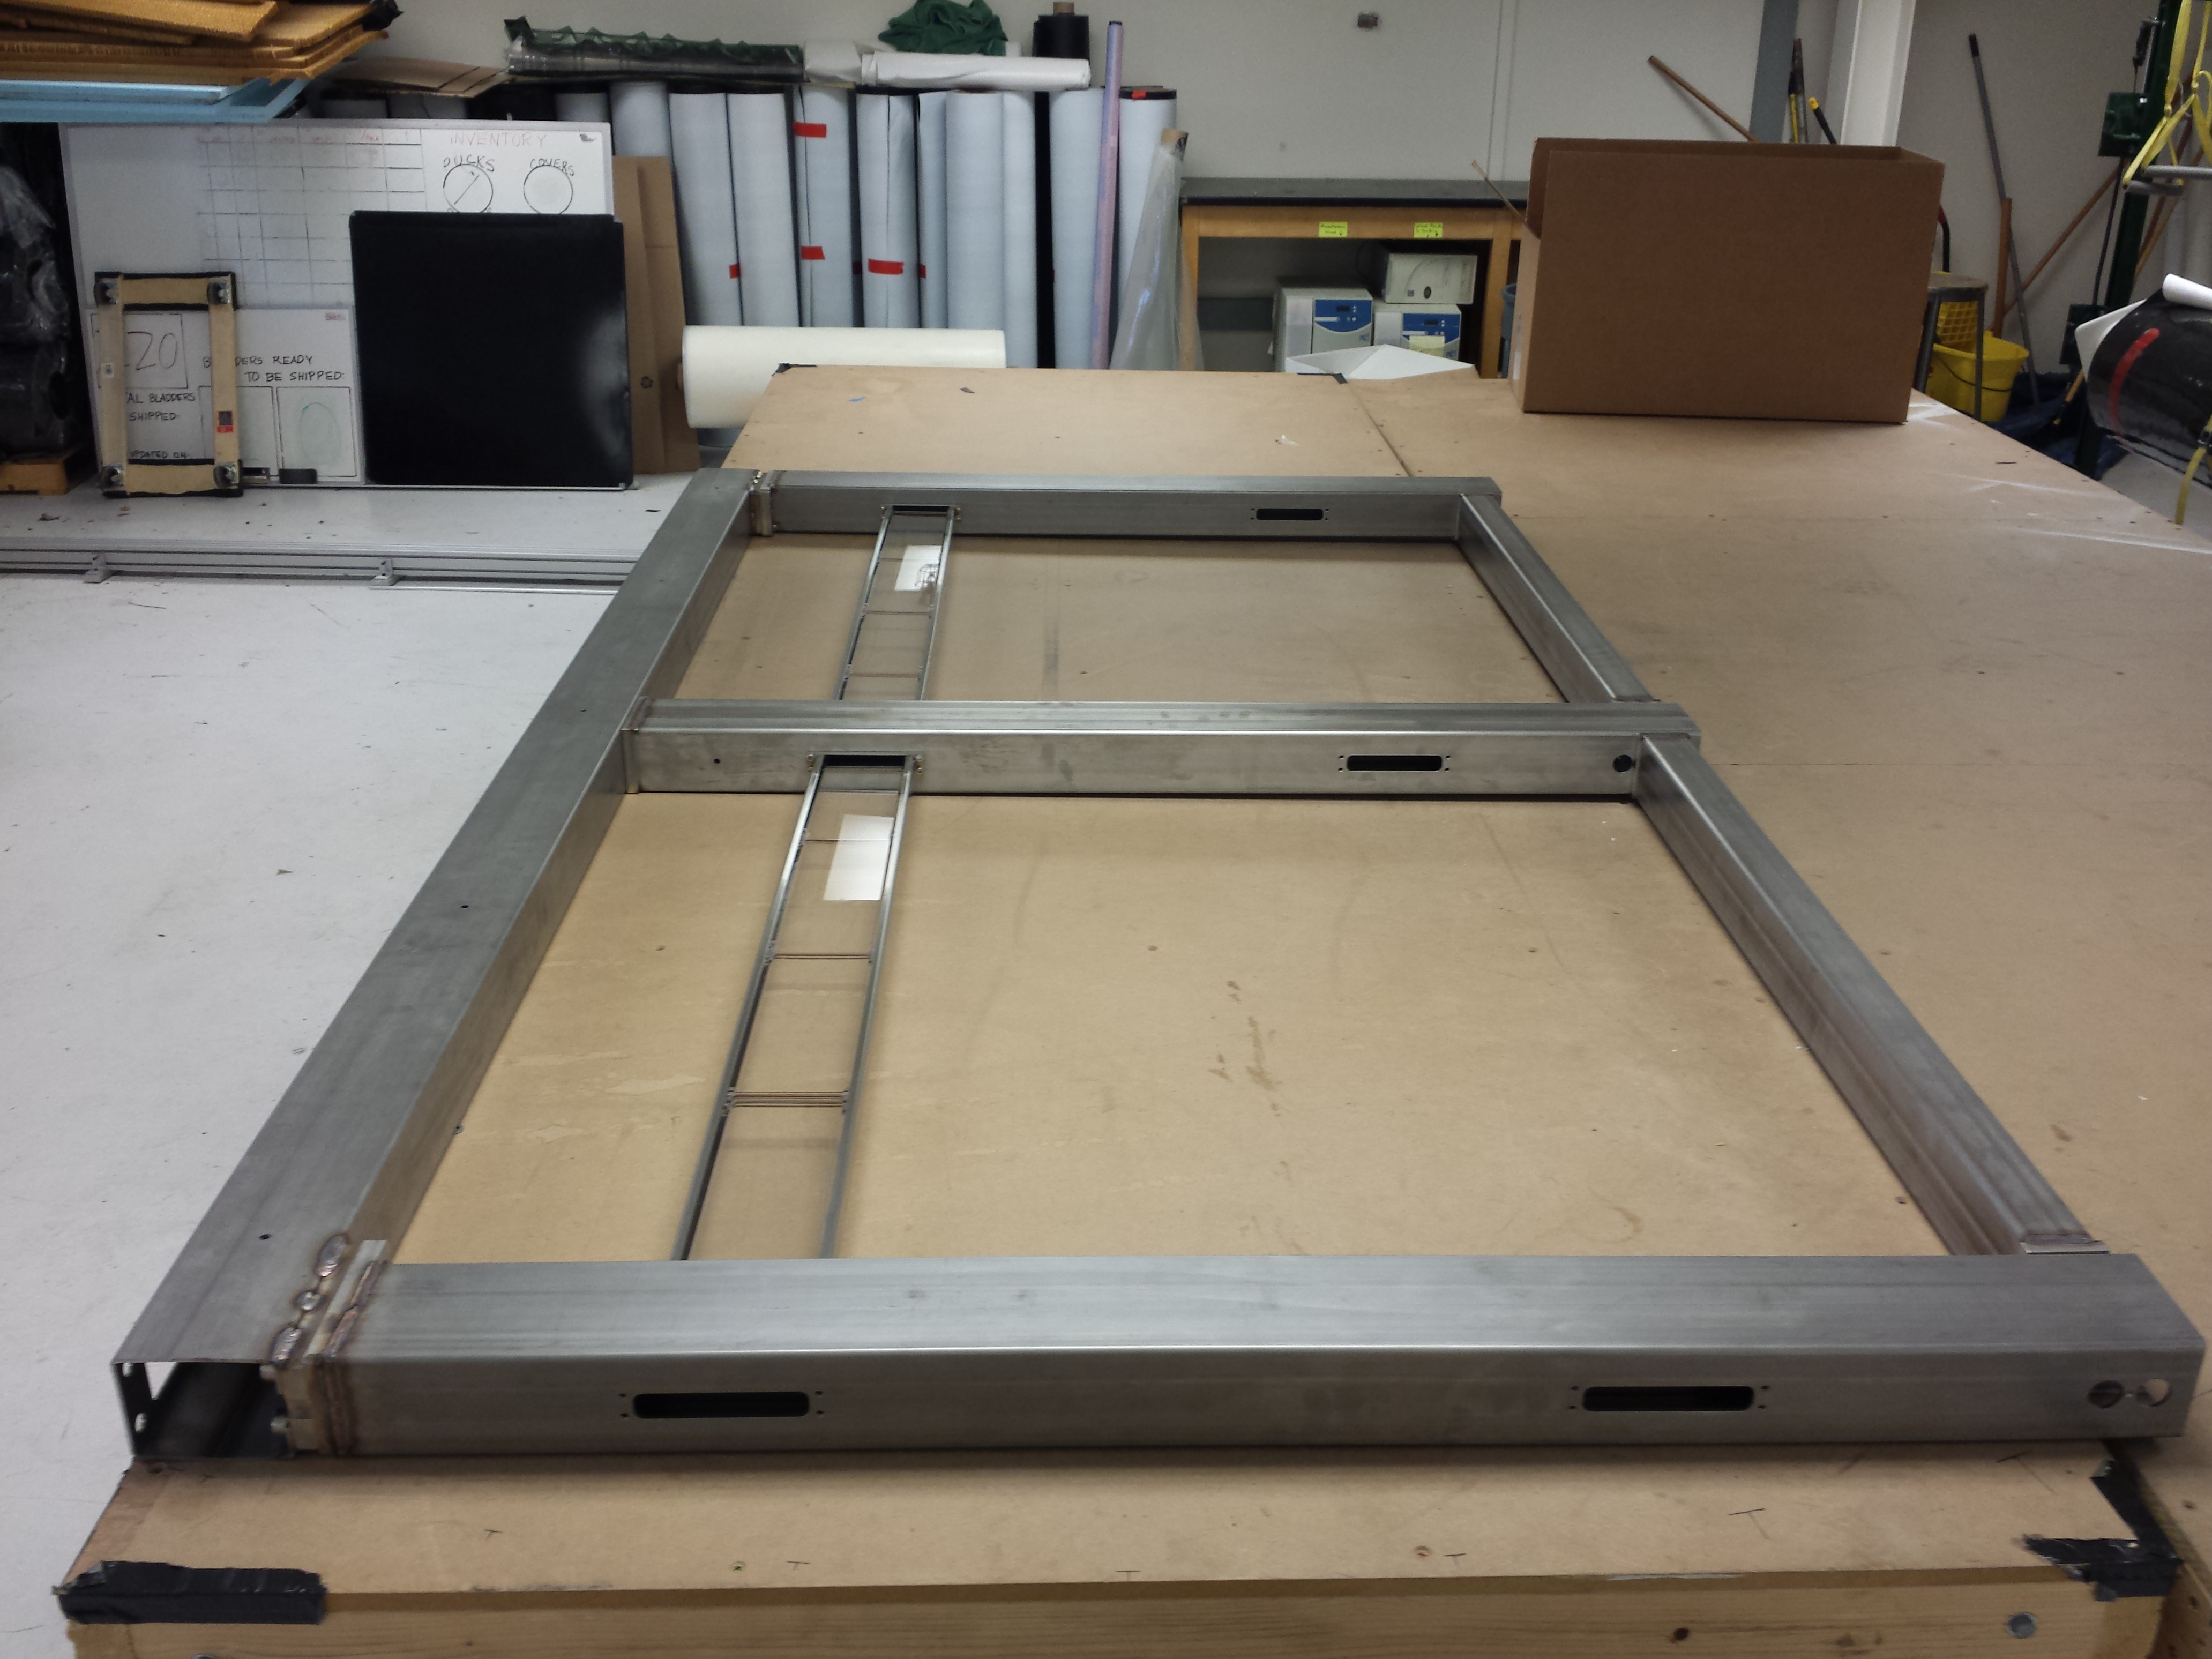
\includegraphics[width=0.50\linewidth]{pd_flat_installtest.jpg}
\end{cdrfigure}

  %   Mechanical Design SiPM mounting board

Each PD has a single SiPM mounting board with 12 surface mount SiPMs 
mounted on the face as in figure~\ref{fig:PD_SiPM_PCB_front}.
There will be four groups of $3$ SiPM elements going to a single 
channel of readout electronics in order to reduce cost of the readout.
The board is held close to the bar, without touching, by four screws that go into 
tapped holes on the end  mounting block that is glued to the bar.  
The mounting block assembly is shown in figure~\ref{fig:PD_endblock_mnt}.
The circuit board also has holes at each end for mounting to the APA frame.  
\begin{cdrfigure}[SiPM Mounting Board with 12 SiPMs mounted]
  {PD_SiPM_PCB_front.PNG}{Photograph of a SiPM mounting board
    with the full complement of 12 SiPMs installed on the board.}
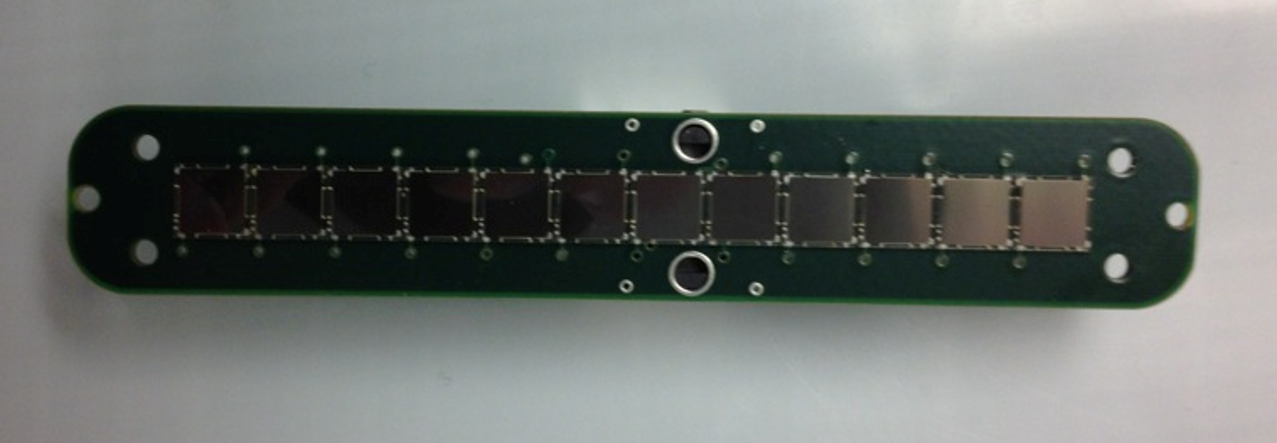
\includegraphics[width=0.50\linewidth]{PD_SiPMMountPCB_front.PNG}
\end{cdrfigure}
\begin{cdrfigure}[SiPM Mounting Board attached to Module]
  {PD_endblock_mnt.PNG}{Rendering of the the SiPM mounting board
    installed on the end of the PD module before insertion.}
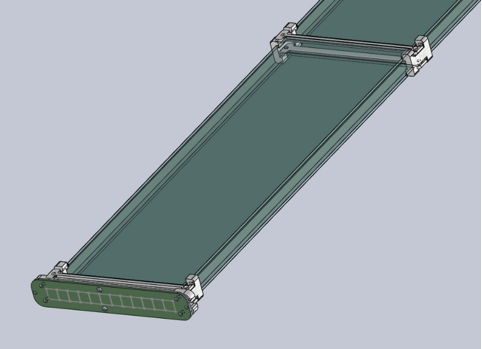
\includegraphics[width=0.50\linewidth]{PD_endblock_mnt.PNG}
\end{cdrfigure}

  %   Mechanical Design Cabling

The cabling plan for the system has one cable with 4 shielded twisted pairs 
connected to each SiPM mounting board via the surface mount RJ-45 connector
shown mounted on the back of the readout PCB in 
figure~\ref{fig:PD_SiPMMountPCB_back.PNG}.  
\begin{cdrfigure}[Readout board with RJ-45 connector]
  {PD_SiPMMountPCB_back}{Photograph of the SiPM readout PCB with the 
    RJ-45 connector for the cable.}
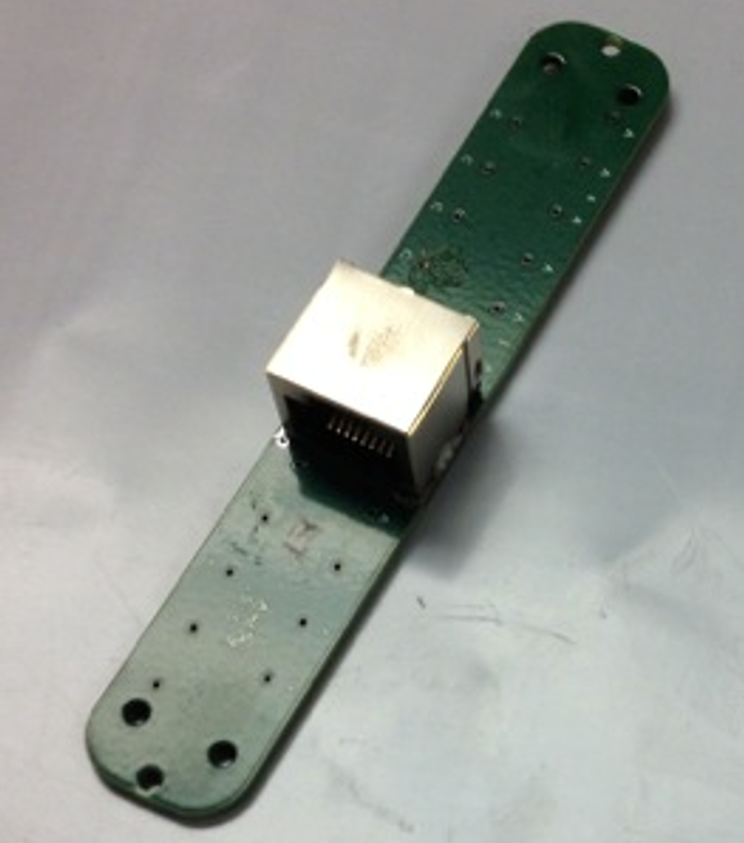
\includegraphics[width=0.50\linewidth]{PD_SiPMMountPCB_back.PNG}
\end{cdrfigure}
The cables run through the APA tubing to the top of the APA frame as seen
in figure~\ref{fig:PD_cable_intube}.
The cable bundles are installed and connected to each PD 
after the PD has been installed into the slot.
\begin{cdrfigure}[Cables in APA frame]
  {PD_cable_intube}{Diagram showing the routing of the PD cables
    through the APA frame.}
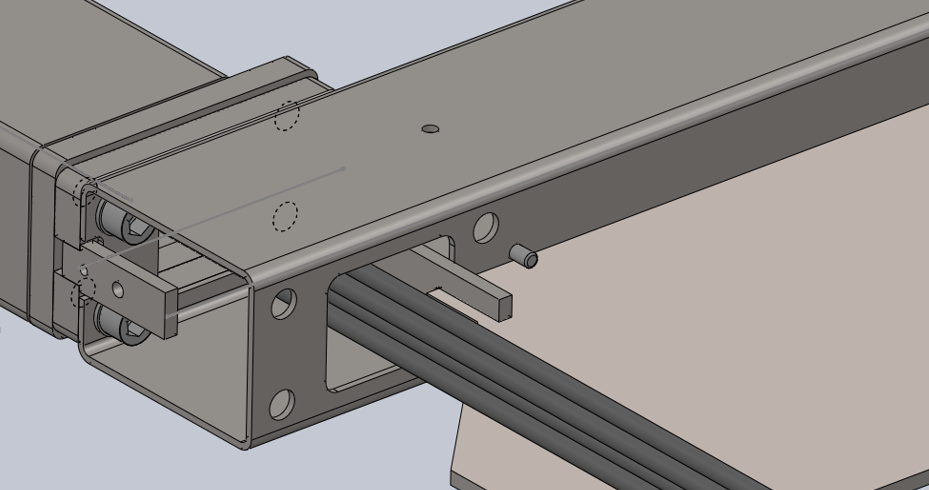
\includegraphics[width=0.50\linewidth]{PD_cable_intube.PNG}
\end{cdrfigure}


%%%%%%%%%%%%%%%%%%%%%%%%%
\subsection{QC Procedures}

  %   QA/QC tracking for components
% This could be a whole document of its own.


